The results of the model independent limits are interpreted in terms of limits
on the fundamental Plank scale in $4 + n$ dimensions (M$_\mathrm{\, D}$) in the
Large Extra Dimensions (LED) scenario proposed by Arkani-Hamed, Dimopoulos and
Dvali (ADD)~\cite{ADDPaper}. In this model, a number of compact extra
dimensions, where only the graviton field is allowed to propagate, are added to
the usual 4 (three spatial dimensions and time) thus effectively reducing the
strength of the gravitational interaction whose scale, M$_\mathrm{\, D}$, could
be at the TeV scale. The generation of the signal and interpretation of the
results follows what was done in the 2015 analysis without major
modifications. Figure~\ref{fig:add_observed} shows the expected and observed
limits at 95\% CL on M$_\mathrm{\, D}$ as a function of the large extra
dimensions $n$. The dashed blue line shows the expected limits using $36.1~\ifb$
with the $\pm 1~\sigma$ and $\pm 2 \sigma$ error bands (green and yellow band
respectively). The red solid line is the observed limit. The limits for
$3.2~\ifb$ are also reported for comparison. Values of M$_\mathrm{\, D}$ up to
7.75~TeV for n = 2 dimensions and 4.8~TeV for n = 6 dimensions are excluded at
95\%~CL improving previous results. The limits where a
M$^4_\mathrm{\, D} / \hat{s}^2$ weighting factor is applied to the visible cross
section for events with $\hat{s} > $ M$^2_\mathrm{\, D}$ (truncation) where
$\hat{s}$ is the center of mass energy of the interacting partons is also
reported in parentheses; the effect of the the truncation is only noticeable in
the ADD n = 6 model meaning that the analysis is probing values of
M$_\mathrm{\, D}$ where the effective theory can be trusted.
\begin{table}[!hb]
  \centering
  \begin{tabular}{lcc}
    \toprule
    \multicolumn{3}{c}{95\% CL Limits on M$_\mathrm{\, D}$
    [TeV]} \\
    \midrule \midrule \\
    ADD Model & Expected & Observed (damped) \\
    n = 2 & 9.27$^{+0.79}_{-0.96}$ & 7.75$^{+0.45}_{-0.55}$ (7.75) \B \\
    n = 3 & 7.13$^{+0.48}_{-0.59}$ & 6.22$^{+0.36}_{-0.47}$ (6.22) \T \B \\
    n = 4 & 6.09$^{+0.34}_{-0.43}$ & 5.49$^{+0.32}_{-0.45}$ (5.49) \T \B \\
    n = 5 & 5.55$^{+0.27}_{-0.32}$ & 5.11$^{+0.30}_{-0.46}$ (5.11) \T \B \\
    n = 6 & 5.20$^{+0.22}_{-0.26}$ & 4.80$^{+0.26}_{-0.47}$ (4.78) \T \\
    \bottomrule
  \end{tabular}
  \caption{Expected and observed 95\% CL lower limits on the fundamental Plank
      scale M$_\mathrm{\, D}$ in $4 + n$ dimensions as a function of the number
      of extra dimensions $n$. The impact of the $\pm 1 \sigma$ uncertainty from
      the theory on the observed limits and the expected $\pm 1 \sigma$ range of
      limits in absence of a signal is reported. The 95\% CL observed limits
      after damping the signal cross section for $\hat{s} > M_D^2$ are also
      reported in parentheses.}
  \label{tab:add_limits}
\end{table}
\begin{figure}[!h]
  \centering
  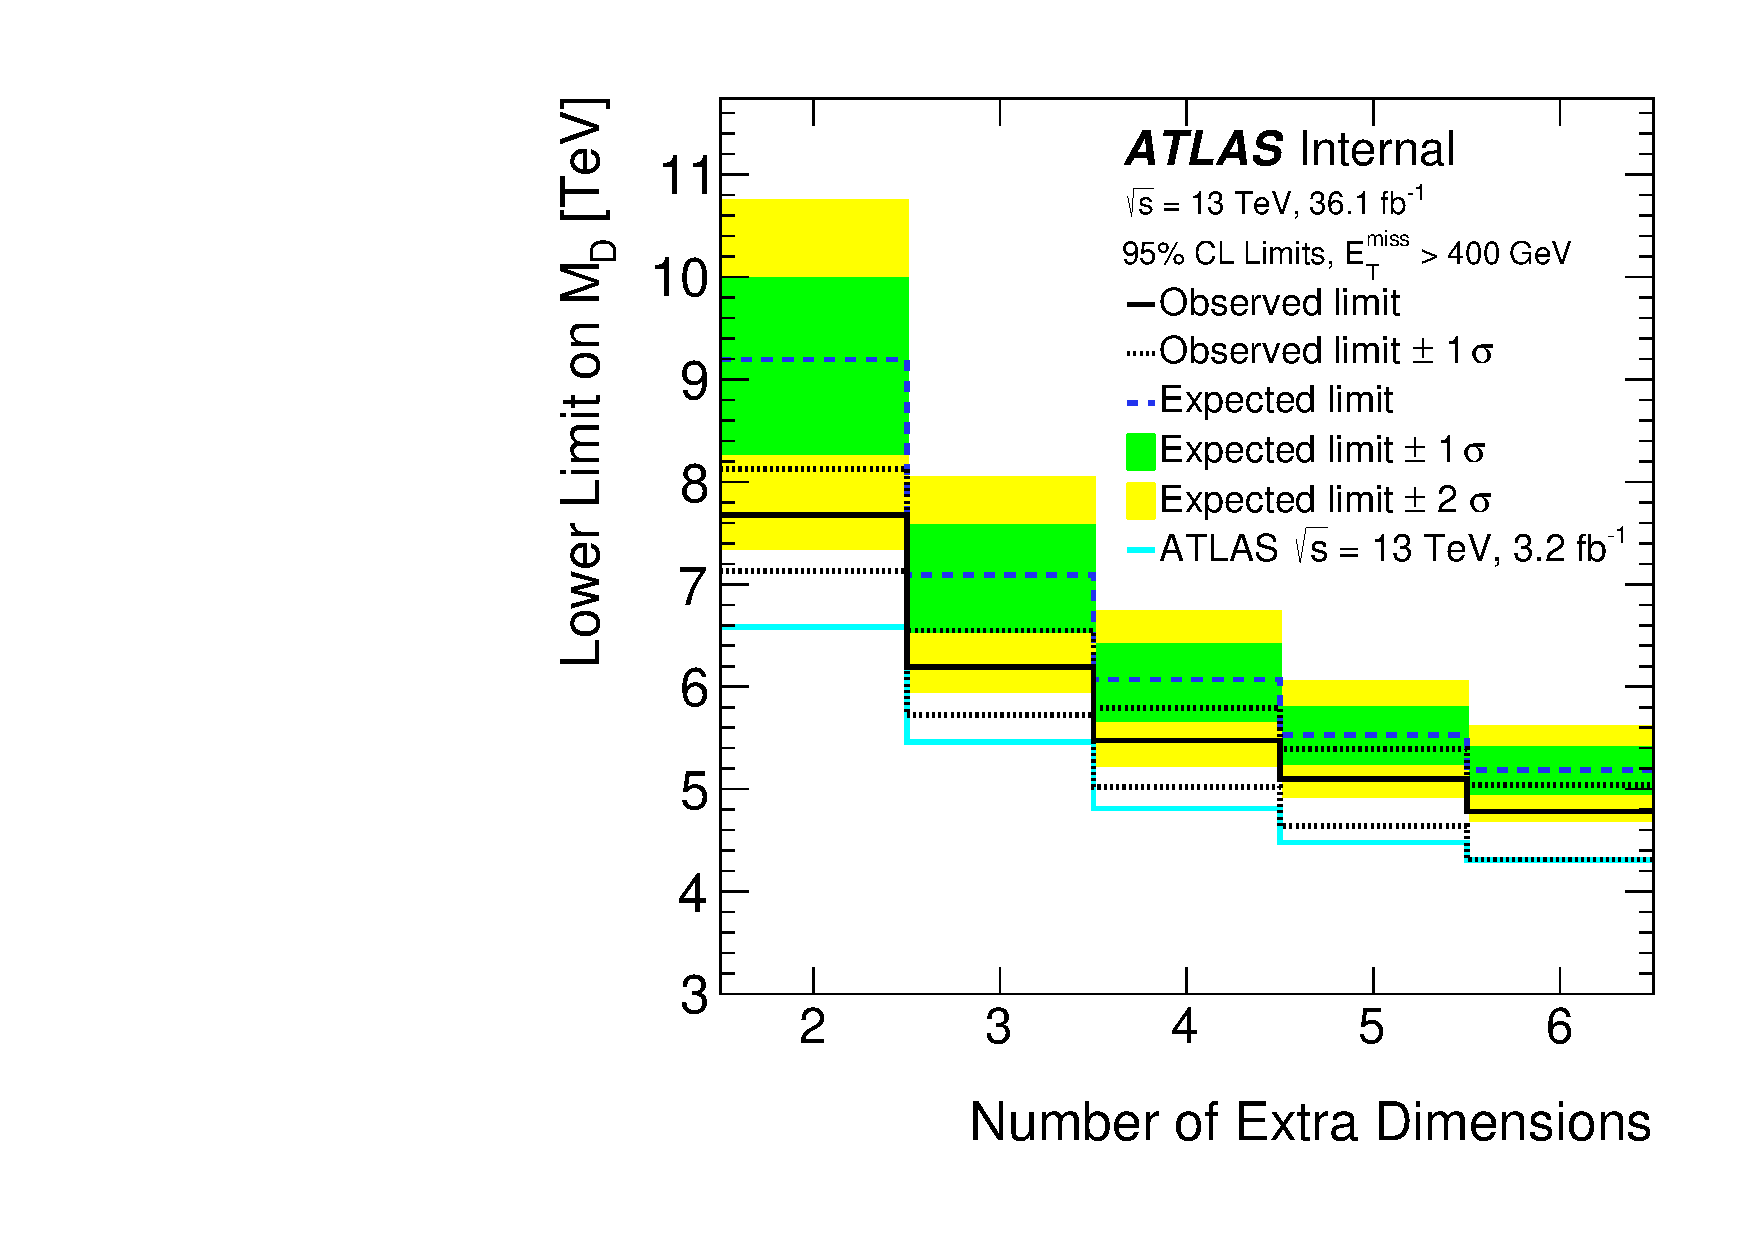
\includegraphics[width=10cm]{add_exclusion_observed}
  \caption{Expected and observed limits at 95\% CL on the fundamental Planck
    Scale in $4 + n$ dimensions, M$_\mathrm{\, D}$, as a function of the number
    of extra dimensions $n$. The dashed blue line shows the expected limit using
    $36.5~\ifb$, the yellow band is the $\pm~1\sigma$ on the estimate. The solid
    red line is the observed limit with the suppression of the $\hat{s} >$
    M$_\mathrm{\, D}^2$ events (truncation) while the cyan line represents the
    observed limits in the 2015 analysis using $3.2~\ifb$.}
  \label{fig:add_observed}
\end{figure}
%%% Local Variables:
%%% mode: latex
%%% TeX-master: "../search_for_DM_LED_with_ATLAS"
%%% End:
